\documentclass[12pt,a4paper]{article}

% ---------- Page geometry as per GNDEC synopsis spec ----------
% left 3.5cm, top 2.5cm, right 1.25cm, bottom 1.25cm
\usepackage[left=3.5cm,top=2.5cm,right=1.25cm,bottom=1.25cm]{geometry}

\usepackage[T1]{fontenc}
\usepackage{mathptmx}           % Times Roman look-alike text+math font
\usepackage{setspace}
\usepackage{graphicx}
\usepackage{tabularx}
\usepackage{booktabs}
\usepackage{enumitem}
\usepackage{titlesec}
\PassOptionsToPackage{hyphens}{url}
\usepackage{hyperref}
\usepackage{tikz}
\usetikzlibrary{arrows.meta, positioning, fit, backgrounds}
\usepackage{microtype}
\usepackage{caption}
\captionsetup{labelfont={it,bf}, textfont=it, font=it}
\renewcommand{\figurename}{Fig.}
\counterwithin{figure}{section}
\sloppy
\emergencystretch=2.5em

\hypersetup{
  colorlinks=true,
  linkcolor=black,
  citecolor=black,
  urlcolor=blue,
  pdftitle={Project Synopsis - Industrial Training TR-104},
  pdfauthor={Gurpiyar Singh}
}

\titleformat{\section}{\bfseries\large}{\thesection}{0.6em}{}
\titleformat{\subsection}{\bfseries\normalsize}{\thesubsection}{0.6em}{}

\setlength{\parindent}{0pt}
\setlength{\parskip}{6pt}

\begin{document}

% ======================================================================
% TITLE PAGE (matches the sample inner-cover sheet supplied by the college)
% ======================================================================
\begin{titlepage}
\centering
\vspace*{1.2cm}

{\fontsize{24}{28}\selectfont\bfseries CLOUD-NATIVE MICROSERVICES\\
PLATFORM WITH CI/CD AND\\
OBSERVABILITY\par}

\vspace{0.6cm}

{\fontsize{14}{18}\selectfont\bfseries PROJECT SYNOPSIS\par}
{\fontsize{12}{16}\selectfont OF INDUSTRIAL TRAINING (TR-104)\par}

\vspace{1.0cm}

{\fontsize{14}{18}\selectfont\bfseries BACHELOR OF TECHNOLOGY\par}
{\fontsize{16}{20}\selectfont COMPUTER SCIENCE ENGINEERING\par}

\vspace{1.2cm}

{\fontsize{14}{18}\selectfont\bfseries SUBMITTED BY\par}
{\fontsize{14}{18}\selectfont\bfseries Gurpiyar Singh\par}
{\fontsize{14}{18}\selectfont\bfseries URN: 2302529\par}

\vspace{1.4cm}

% ---- Replace this frame with the actual GNDEC logo image ----
\includegraphics[height=5.5cm]{gne\_logo.png}\\
%\fbox{\parbox[c][3.5cm][c]{3.5cm}{\centering\itshape GNDEC\\LOGO}}

\vspace{1.2cm}

{\fontsize{16}{20}\selectfont\bfseries GURU NANAK DEV ENGINEERING COLLEGE,\\
LUDHIANA\par}

\vfill
\end{titlepage}

% ======================================================================
% CANDIDATE / TRAINING DETAILS PAGE
% (the seven title-page items called for by the department format sheet)
% ======================================================================
\section*{Candidate and Training Details}

\noindent\textbf{1. Name of Student:} Gurpiyar Singh

\noindent\textbf{2. PTU (University) Roll No.:} 2302529

\noindent\textbf{3. Class Roll No.:} 2315072

\noindent\textbf{4. Present Official Address:} AppSmartz, 2nd Floor, Quark City,
Sector 75, Mohali, Punjab, India 160059 --- E-mail:
gurpiyar656@gmail.com, Telephone: +91-9803822976

\noindent\textbf{5. Branch:} Computer Science Engineering

\noindent\textbf{6. Batch:} 2023--2027

\noindent\textbf{7. Proposed Topic:} Cloud-Native Microservices Platform with CI/CD and Observability

\vspace{0.6cm}
\hrule
\vspace{0.4cm}

\noindent\textbf{Training Organization:} AppSmartz

\noindent\textbf{Duration of Training:} 29-06-2026 to 31-12-2026

\noindent\textbf{Organization Mentor:} Mr. Harshdeep Singla, Tech Lead

\noindent\textbf{College Guide:} Prof. Shailja

\noindent\textbf{Live Deployment:} \url{https://learning.run.place}

\newpage

% ======================================================================
% INDEX
% ======================================================================
\tableofcontents
\newpage

\onehalfspacing
\doublespacing

% ======================================================================
\section{Introduction}
% (should not exceed 3 pages)
% ======================================================================

\subsection{Background and Motivation}

My industrial training at AppSmartz was spent with the backend/DevOps team,
observing at close quarters the mechanics by which software transitions from a
developer's workstation to a resilient, production-grade system: decomposition
into loosely-coupled services, automated integration and delivery, traffic
arbitration through a reverse proxy, and continuous instrumentation of the
running system's health. This synopsis proposes a project that condenses that
entire lifecycle into a scale tractable for a training period, while retaining
the fidelity of the underlying paradigm -- architecture, containerization,
CI/CD, secure public exposure, and observability are all genuinely implemented,
not merely narrated.

\subsection{System Architecture Overview}

The platform itself is an e-commerce-style system decomposed into twelve
independent, single-responsibility Node.js/Express microservices --
\texttt{user}, \texttt{product}, \texttt{order}, \texttt{cart},
\texttt{inventory}, \texttt{payment}, \texttt{notification}, \texttt{review},
\texttt{auth}, \texttt{shipping}, \texttt{search} and \texttt{analytics} --
each encapsulating its own data and its own \texttt{Dockerfile}. None is
exposed externally; every inbound request is arbitrated by a single
\textbf{API Gateway}, which proxies each \texttt{/api/\ldots} route to its
corresponding service and presents one coherent surface to the outside world.
A \textbf{frontend dashboard} renders this surface as a live health-check
grid, an animated request console, and reactive data tables, while the API
contract is formalised as an \textbf{OpenAPI 3} specification and exposed
interactively through \textbf{Swagger UI} at \texttt{/api-docs}.

\subsection{Automated Build and Delivery Pipeline}

Delivery is fully automated. Every service is containerized with
\textbf{Docker}; \textbf{Docker Compose} orchestrates the ensemble, with a
development variant that builds images from source and a production variant
that pulls immutable, pre-built artifacts. Bridging the two is a
\textbf{Jenkins} pipeline that checks out the repository, runs the codebase
through a \textbf{SonarQube} static-analysis quality gate to catch
maintainability and security issues before they compound, builds and tags an
image per service, pushes those images to Docker Hub, and finally deploys the
production stack to the remote host over SSH -- a declarative sequence that
removes the human from the critical path between a commit and a release.

\subsection{Secure Hosting and Observability}

Two capabilities are being layered onto this foundation specifically because
of practices observed at AppSmartz that had not previously been attempted: a
\textbf{secured public domain} and a \textbf{dedicated observability stack}.
The platform is reachable at \url{https://learning.run.place} through an
\textbf{Nginx} reverse proxy terminating \textbf{TLS/SSL} via a Let's
Encrypt/Certbot certificate, so the system is a genuine HTTPS deployment
rather than a \texttt{localhost} artefact. Alongside it, \textbf{Prometheus}
scrapes request-rate, latency and error telemetry from every service,
\textbf{Promtail} ships container logs into \textbf{Grafana Loki} for
centralised aggregation, and \textbf{Grafana} dashboards unify both signals
so the cluster's behaviour is legible from a single pane rather than
reconstructed service by service. Together, static analysis, encrypted
ingress and full-stack telemetry are what separate a demo from a platform --
and, should the mesh outgrow a single Compose deployment, the same
container images translate directly onto an orchestrator such as
\textbf{Kubernetes} without modification.

\subsection{Glossary of Key Terms}

A brief glossary for terms used throughout: a \textbf{microservice} is a
small, independently deployable unit owning one business capability; an
\textbf{API gateway} unifies many such services behind one address; a
\textbf{reverse proxy} accepts public traffic and forwards it internally
while handling cross-cutting concerns such as TLS termination; a
\textbf{CI/CD pipeline} automates the path from a code change to a running
deployment; a \textbf{quality gate} (SonarQube, here) blocks a build that
fails defined code-health thresholds; and \textbf{observability} denotes the
ability to reason about a running system from its metrics, logs and traces
rather than by inference.

% ======================================================================
\clearpage
\section{Feasibility Study}
% (should not exceed 1 page)
% ======================================================================

\subsection{Technical Feasibility}

Every tool used in the project -- Node.js,
Express, Docker, Docker Compose, Jenkins, SonarQube, Nginx, Prometheus, Loki
and Grafana -- is open source, widely documented, and already partly proven inside this
project: the fourteen services, the API gateway, the Jenkins pipeline and the
Swagger documentation are already built and run correctly in Docker Compose.
What remains (the Nginx/SSL front door and the Prometheus--Loki--Grafana
stack) uses the same container-based approach as the rest of the project, so
no new deployment model has to be learned, only new containers added to the
same compose file. The images are small (Alpine-based), so the whole stack,
including the monitoring containers, comfortably fits on a single low-cost
cloud instance.

\subsection{Economic Feasibility}

There are no licensing costs anywhere in the
stack -- Docker, Jenkins, SonarQube's Community Edition, Nginx, Prometheus,
Loki and Grafana are all free and open source, and Let's Encrypt issues the
TLS certificate for the domain at no
cost. The only recurring cost is the small VPS the project is hosted on at
\url{https://learning.run.place}, which is well within what a student project
can sustain.

\subsection{Operational Feasibility}

Because the whole stack is defined in a
handful of Compose files and a Jenkinsfile, standing it up, tearing it down,
or moving it to a different server is a small number of documented commands
rather than a manual, error-prone process. The health-check dashboard and,
once added, the Grafana dashboards mean that a problem with any one of the
fourteen services is visible immediately rather than discovered from a user
complaint.

\subsection{Need and Significance}

College coursework covers data structures,
databases and individual application development well, but rarely the
question this project is built around: once an application is written, how
does an organisation actually run many pieces of it reliably, ship changes to
it safely, and know when something has gone wrong? That gap is exactly what
this training placement, and this project, are meant to close -- it takes the
CI/CD, containerization, reverse-proxy and observability practices seen at
AppSmartz and turns them into a working system I can point to and explain,
rather than a slide describing them.

% ======================================================================
\clearpage
\section{Methodology / Planning of Work}
% (should not exceed 1 page)
% ======================================================================

\subsection{Development Stages}

The work is organised as a sequence of stages, most already completed and the
remainder planned for the rest of the training period:

\begin{enumerate}[label=\arabic*., itemsep=2pt, topsep=2pt]
  \item \textbf{Requirement analysis and service decomposition} -- identify the
        independent business capabilities (users, products, orders, cart,
        inventory, payments, notifications, reviews, auth, shipping, search,
        analytics) and give each its own service boundary and data.
  \item \textbf{Service development} -- implement each service as a small
        Express application exposing a REST API and a \texttt{/health}
        endpoint used later by both the dashboard and Prometheus.
  \item \textbf{API Gateway} -- build a single Express-based gateway that
        proxies \texttt{/api/*} routes to the correct service, so the outside
        world only ever talks to one address.
  \item \textbf{Containerization} -- write a \texttt{Dockerfile} per service
        and two Compose files: one that builds every service from source for
        local development, one that pulls tagged images for deployment.
  \item \textbf{API documentation} -- write an OpenAPI 3 specification
        covering every route and serve it as an interactive Swagger UI from
        the gateway at \texttt{/api-docs}.
  \item \textbf{CI/CD pipeline} -- a Jenkinsfile that checks the repository
        out, runs a \textbf{SonarQube} static-analysis quality gate on the
        codebase, builds and tags a Docker image per service, pushes the
        images to Docker Hub, and deploys the production compose file to the
        server over SSH.
  \item \textbf{Public hosting with TLS} -- point the domain
        \url{https://learning.run.place} at the deployment server and put an
        Nginx reverse proxy in front of the frontend/gateway, terminating
        HTTPS with a Let's Encrypt certificate and redirecting plain HTTP to
        HTTPS.
  \item \textbf{Observability stack} -- add Prometheus to scrape metrics from
        the gateway and every service, Promtail to ship container logs into
        Loki, and Grafana dashboards that bring request rate, latency, error
        rate and searchable logs together in one place.
  \item \textbf{Testing} -- exercise every endpoint through the Swagger UI and
        the dashboard's request console, and confirm the health grid, the
        Grafana dashboards and the HTTPS certificate all behave correctly
        under normal and failure conditions (e.g. a service stopped
        deliberately).
  \item \textbf{Documentation and submission} -- record the final
        architecture and write up this synopsis and the subsequent training
        report.
\end{enumerate}

\subsection{System Architecture Diagram}

The overall request path, the CI/CD path and the observability path that
result from these stages are shown together in Fig.~\ref{fig:architecture}.

\begin{figure}[h]
\centering
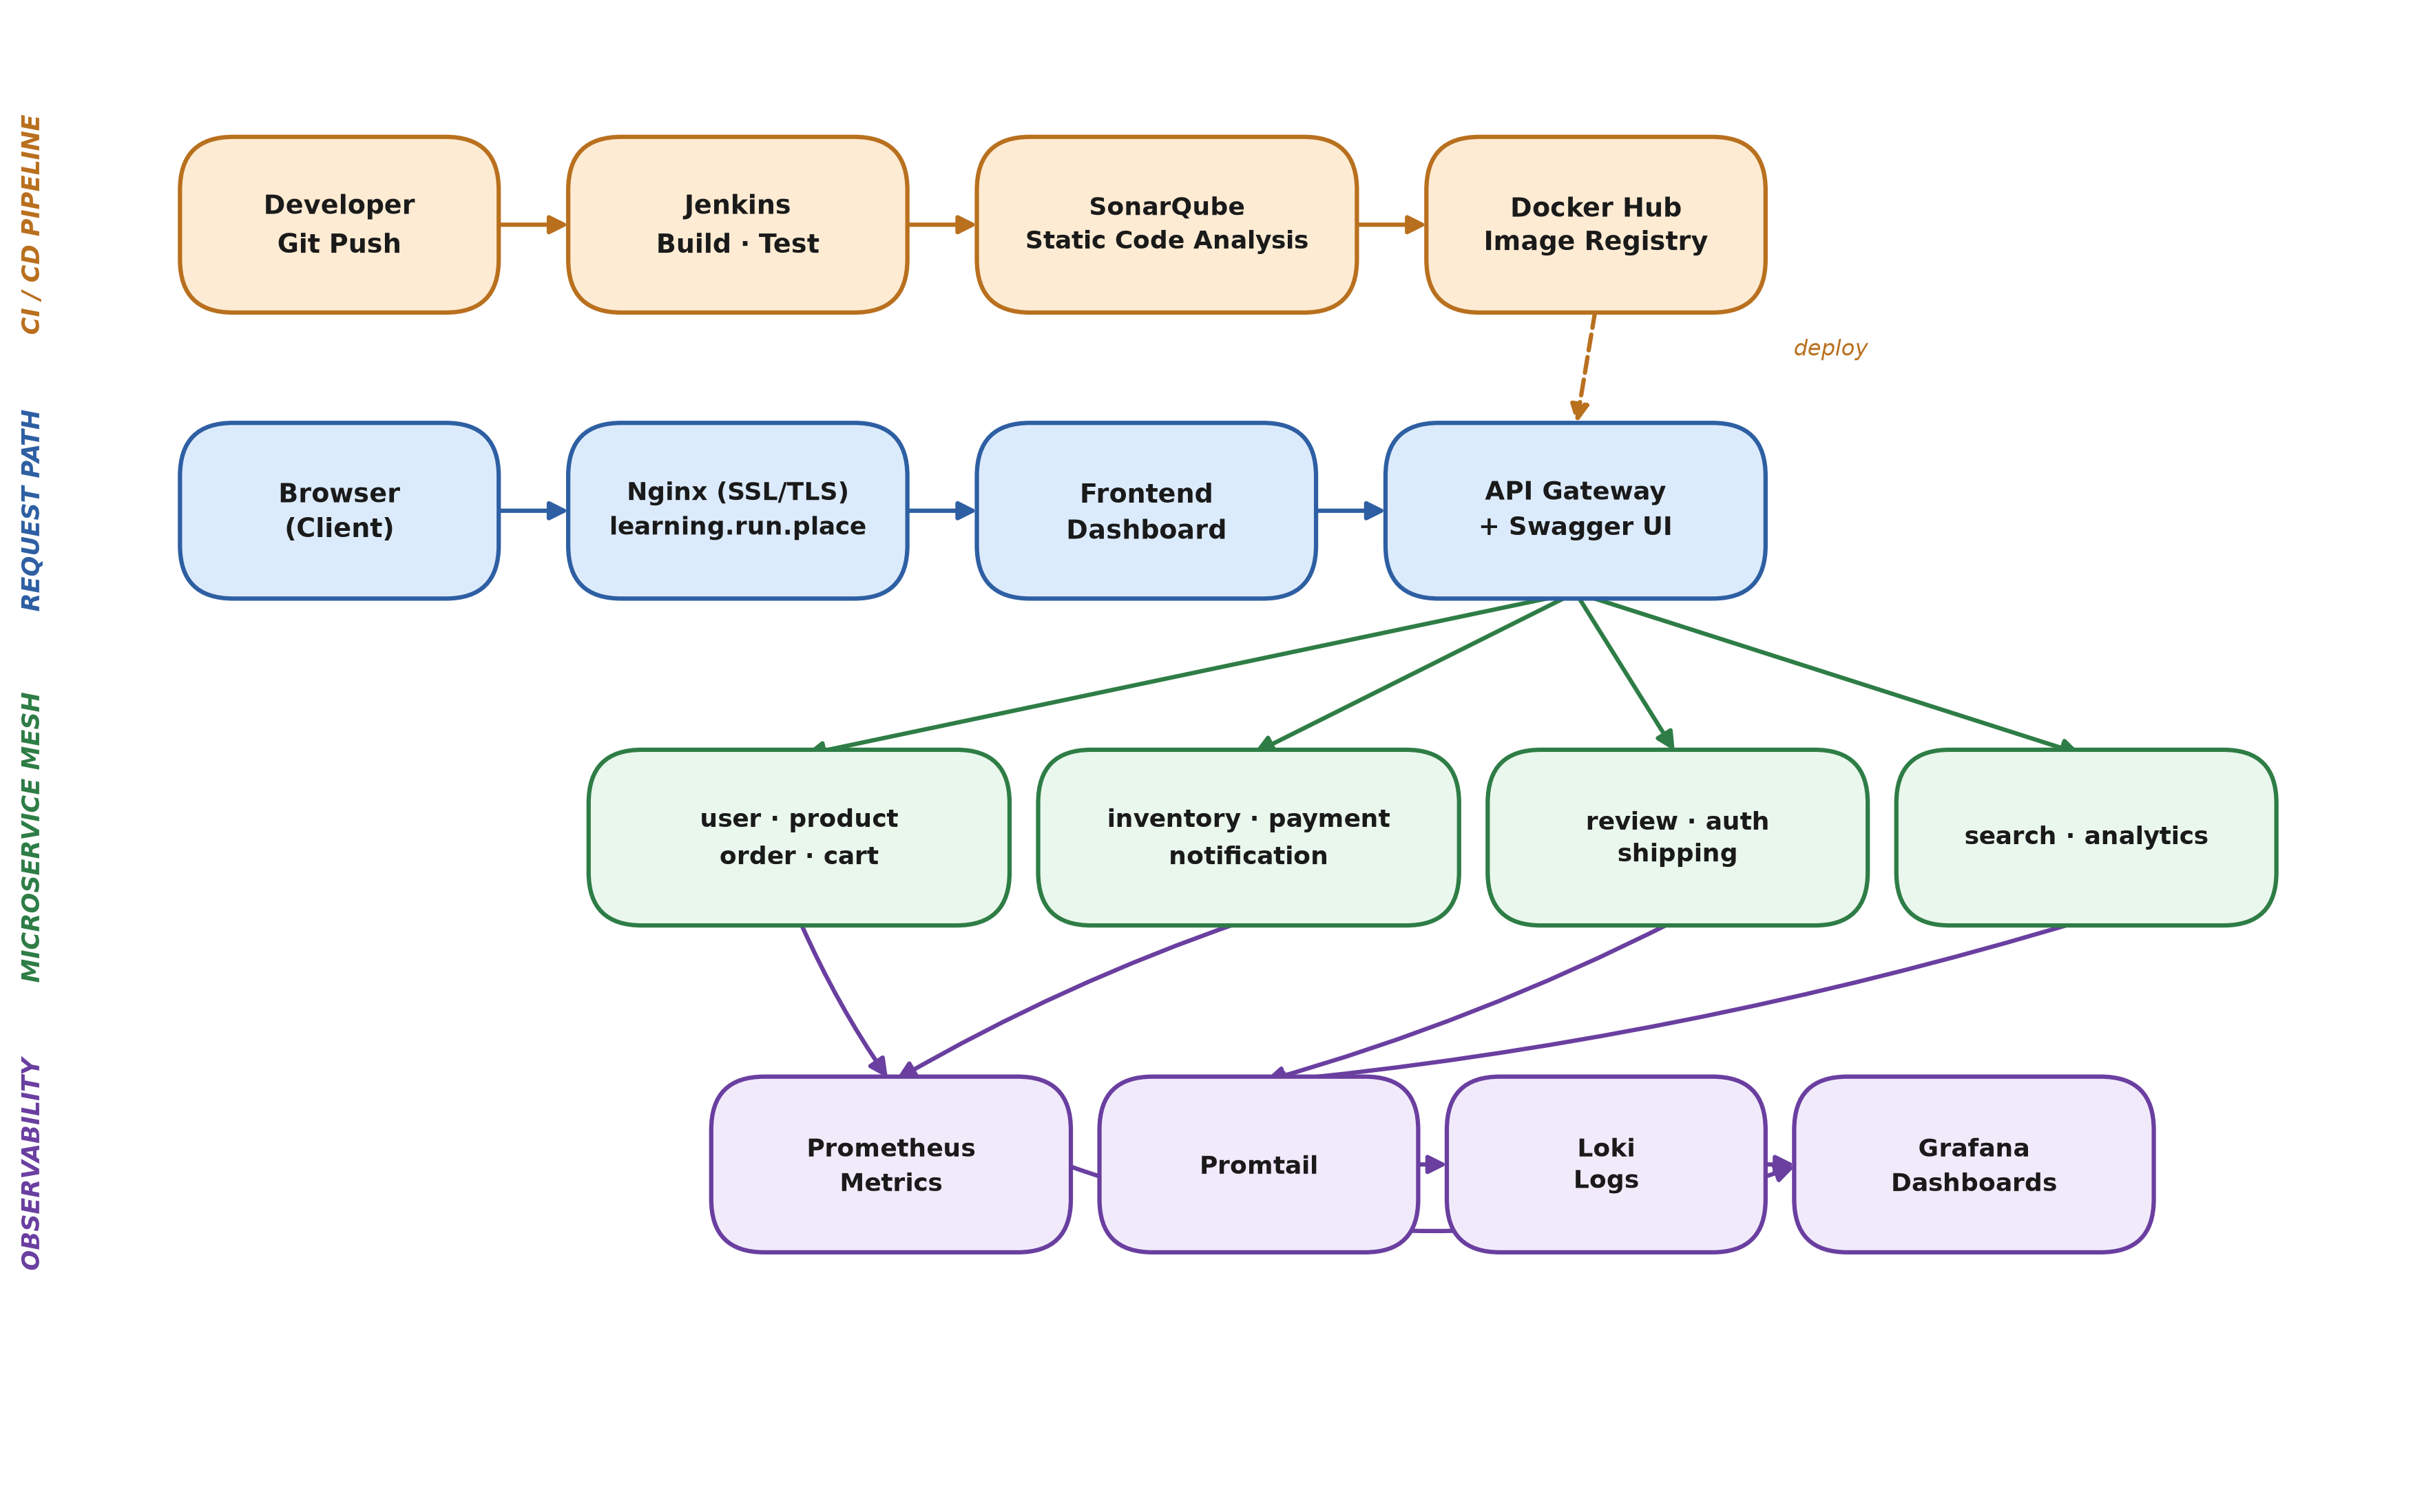
\includegraphics[width=\linewidth]{architecture.png}
\caption{CI/CD pipeline with the SonarQube quality gate (top), request path (middle), the microservice mesh, and the observability path (bottom).}
\label{fig:architecture}
\end{figure}

% ======================================================================
\clearpage
\section{Facilities Required for Proposed Work}
% ======================================================================

\subsection{Software}
\begin{itemize}[itemsep=1pt, topsep=2pt]
  \item Node.js and Express.js -- backend services and API gateway
  \item Docker and Docker Compose -- containerization and local orchestration
  \item Jenkins -- CI/CD pipeline (build, push, deploy)
  \item SonarQube -- static code analysis and quality gate
  \item Nginx and Certbot (Let's Encrypt) -- reverse proxy and TLS for \url{https://learning.run.place}
  \item Prometheus -- metrics collection
  \item Grafana Loki and Promtail -- centralised log aggregation
  \item Grafana -- dashboards and visualisation
  \item Swagger UI / OpenAPI 3 -- API documentation
  \item Git and GitHub -- version control
  \item Visual Studio Code -- development environment
\end{itemize}

\subsection{Hardware}
\begin{itemize}[itemsep=1pt, topsep=2pt]
  \item Development laptop (minimum 8 GB RAM) for local Docker Compose builds
  \item A cloud VPS (Ubuntu, 2 vCPU / 4 GB RAM or better) hosting the domain
        \url{https://learning.run.place}
  \item Stable internet connectivity for pushing/pulling container images and
        remote deployment
\end{itemize}

% ======================================================================
\clearpage
\section*{Bibliography}
\addcontentsline{toc}{section}{Bibliography}
% ======================================================================

\begin{enumerate}[leftmargin=1.4cm, itemsep=3pt]
  \item Docker Inc., \emph{Docker Documentation}, \url{https://docs.docker.com}
  \item Docker Inc., \emph{Docker Compose Documentation}, \url{https://docs.docker.com/compose/}
  \item Jenkins Project, \emph{Jenkins User Documentation}, \url{https://www.jenkins.io/doc/}
  \item SonarSource, \emph{SonarQube Documentation}, \url{https://docs.sonarsource.com/sonarqube/latest/}
  \item Nginx Inc., \emph{Nginx Documentation}, \url{https://nginx.org/en/docs/}
  \item Electronic Frontier Foundation, \emph{Certbot / Let's Encrypt Documentation}, \url{https://certbot.eff.org}
  \item Prometheus Authors, \emph{Prometheus Documentation}, \url{https://prometheus.io/docs/}
  \item Grafana Labs, \emph{Grafana Documentation}, \url{https://grafana.com/docs/grafana/latest/}
  \item Grafana Labs, \emph{Loki Documentation}, \url{https://grafana.com/docs/loki/latest/}
  \item OpenAPI Initiative, \emph{OpenAPI Specification v3.0}, \url{https://spec.openapis.org/oas/v3.0.3}
  \item SmartBear Software, \emph{Swagger UI Documentation}, \url{https://swagger.io/tools/swagger-ui/}
  \item OpenJS Foundation, \emph{Express.js Documentation}, \url{https://expressjs.com}
  \item Sam Newman, \emph{Building Microservices}, 2nd Edition, O'Reilly Media, 2021.

\end{enumerate}

\end{document}
